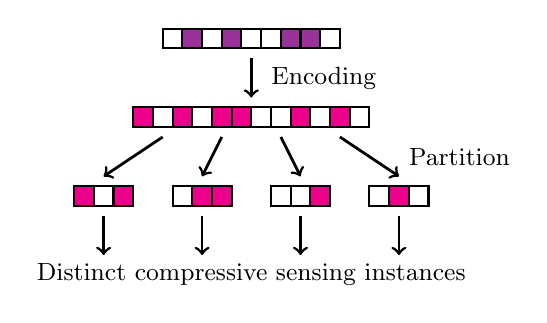
\begin{tikzpicture}
[font=\small, draw=black, line width=0.75pt,
bit0/.style={rectangle, draw, inner sep=0pt, minimum size=2.5mm},
bit1/.style={rectangle, draw, fill=violet!80, inner sep=0pt, minimum size=2.5mm},
ebit0/.style={rectangle, draw, inner sep=0pt, minimum size=2.5mm},
ebit1/.style={rectangle, draw, fill=magenta, inner sep=0pt, minimum size=2.5mm}
]

\node[bit0] (info0) at (0.875,5) {};
\node[bit1] (info1) at (1.125,5) {};
\node[bit0] (info2) at (1.375,5) {};
\node[bit1] (info3) at (1.625,5) {};
\node[bit0] (info4) at (1.875,5) {};
\node[bit0] (info5) at (2.125,5) {};
\node[bit1] (info6) at (2.375,5) {};
\node[bit1] (info7) at (2.625,5) {};
\node[bit0] (info8) at (2.875,5) {};

\draw[->, line width=1pt]  (1.875,4.75) -- (1.875,4.25);
\node[anchor=west] (coding) at (2,4.50) {Encoding};

\node[ebit1] (ebit0) at (0.50,4) {};
\node[ebit0] (ebit1) at (0.75,4) {};
\node[ebit1] (ebit2) at (1.00,4) {};
\node[ebit0] (ebit3) at (1.25,4) {};
\node[ebit1] (ebit4) at (1.50,4) {};
\node[ebit1] (ebit5) at (1.75,4) {};
\node[ebit0] (ebit6) at (2.00,4) {};
\node[ebit0] (ebit7) at (2.25,4) {};
\node[ebit1] (ebit8) at (2.50,4) {};
\node[ebit0] (ebit9) at (2.75,4) {};
\node[ebit1] (ebit10) at (3.00,4) {};
\node[ebit0] (ebit11) at (3.25,4) {};

\draw[->, line width=1pt]  (0.75,3.75) -- (0.00,3.25);
\draw[->, line width=1pt]  (1.50,3.75) -- (1.25,3.25);
\draw[->, line width=1pt]  (2.25,3.75) -- (2.50,3.25);
\draw[->, line width=1pt]  (3.00,3.75) -- (3.75,3.25);
\node[anchor=west] (coding) at (3.75,3.50) {Partition};

\node[ebit1] (s00) at (-0.25,3.00) {};
\node[ebit0] (s01) at (0.00,3.00) {};
\node[ebit1] (s02) at (0.25,3.00) {};

\node[ebit0] (s03) at (1.00,3.00) {};
\node[ebit1] (s04) at (1.25,3.00) {};
\node[ebit1] (s05) at (1.50,3.00) {};

\node[ebit0] (s06) at (2.25,3.00) {};
\node[ebit0] (s07) at (2.50,3.00) {};
\node[ebit1] (s08) at (2.75,3.00) {};

\node[ebit0] (s09) at (3.50,3.00) {};
\node[ebit1] (s10) at (3.75,3.00) {};
\node[ebit0] (s11) at (4.00,3.00) {};

\draw[->, line width=1pt]  (0.00,2.75) -- (0.00,2.25);
\draw[->, line width=1pt]  (1.25,2.75) -- (1.25,2.25);
\draw[->, line width=1pt]  (2.50,2.75) -- (2.50,2.25);
\draw[->, line width=1pt]  (3.75,2.75) -- (3.75,2.25);

\node (cs) at (1.875,2.00) {Distinct compressive sensing instances};
\end{tikzpicture}
